\section{Backend Study Details}
\label{app:backend-details}

The operation census, matched runtime, per-operation, and production verified-mode
experiments use separate frozen cohorts: \path{e6/isolation-v1},
\path{e6/runtime-v1}, \path{e6/operations-v1}, and \path{e6/verified-v2}
under \path{eval/reports/}. Application A/B/C labels do not denote these backend
conditions. Run-level host captures supersede the older hardware summary.
The runtime host uses Python 3.12.3, logical CPU~0, and monotonic
\code{perf\_counter\_ns}; CPU frequency, OS caches, and other host activity are
uncontrolled. GPUs serve no role in the backend timing experiments.

\begin{table*}[t]
\centering
\small
\begin{tabular}{llrrrr}
\toprule
Workload & Condition & Mean (ms) & SD (ms) & Median (ms) & P95 (ms) \\
\midrule
Arithmetic & Trusted & 28.14 & 3.18 & 28.85 & 31.15 \\
 & Helper & 28.14 & 2.98 & 28.99 & 31.59 \\
 & Host & 430.63 & 50.82 & 445.93 & 480.34 \\
 & Host + helper & 428.47 & 50.30 & 445.78 & 476.11 \\
\addlinespace
Read & Trusted & 27.72 & 3.52 & 28.97 & 31.15 \\
 & Helper & 28.10 & 3.43 & 29.09 & 31.27 \\
 & Host & 433.31 & 45.59 & 447.36 & 478.07 \\
 & Host + helper & 431.74 & 49.10 & 448.03 & 481.50 \\
\addlinespace
Write 4 KiB & Trusted & 27.92 & 3.50 & 29.12 & 31.96 \\
 & Helper & 28.16 & 3.26 & 29.09 & 31.50 \\
 & Host & 433.61 & 52.87 & 447.99 & 491.47 \\
 & Host + helper & 431.19 & 49.51 & 446.89 & 481.22 \\
\bottomrule
\end{tabular}
\caption{Synthetic matched backend runtime, 100 successful calls per row.
Setup/preflight is excluded. The helper condition is not production verified mode.}
\label{tab:backend-timing}
\end{table*}

\begin{table*}[t]
\centering
\small
\begin{tabular}{lrrr}
\toprule
 & Host $-$ trusted & Host+helper $-$ helper & Host+helper $-$ host \\
Workload & Mean (SD), ms & Mean (SD), ms & Mean (SD), ms \\
\midrule
Arithmetic & $402.49$ (48.52) & $400.33$ (48.69) & $-2.16$ (34.06) \\
Read & $405.59$ (43.06) & $403.64$ (46.73) & $-1.57$ (32.98) \\
Write 4 KiB & $405.69$ (50.68) & $403.03$ (47.80) & $-2.43$ (31.65) \\
\bottomrule
\end{tabular}
\caption{Same-round paired increments. Small negative helper differences do not
establish a speedup. Paired SDs are reported directly, not reconstructed from
marginal SDs or used as confidence intervals. Rounded means need not reproduce
every last digit of a full-precision paired estimate.}
\label{tab:backend-paired}
\end{table*}

\begin{table*}[t]
\centering
\small
\begin{tabular}{lrrrrr}
\toprule
Workload & Verified (ms) & Host (ms) & Added mean (ms) & Added SD (ms) & Host/verified \\
\midrule
Constant & 18.479 & 319.774 & 301.295 & 36.116 & $17.31\times$ \\
Read 32 B & 28.466 & 330.207 & 301.740 & 37.792 & $11.60\times$ \\
Read 4 KiB & 27.830 & 331.581 & 303.751 & 34.993 & $11.91\times$ \\
Read 64 KiB & 27.344 & 360.600 & 333.256 & 40.938 & $13.19\times$ \\
Two reads, 32 B & 28.130 & 330.491 & 302.361 & 35.602 & $11.75\times$ \\
\bottomrule
\end{tabular}
\caption{Production-mode comparison, 50 paired successful samples per workload.
Means include each mode's own policy frontend; differences are not a pure
kernel-isolation tax. Added SD describes the paired difference.}
\label{tab:verified-timing}
\end{table*}

\begin{figure*}[t]
  \centering
  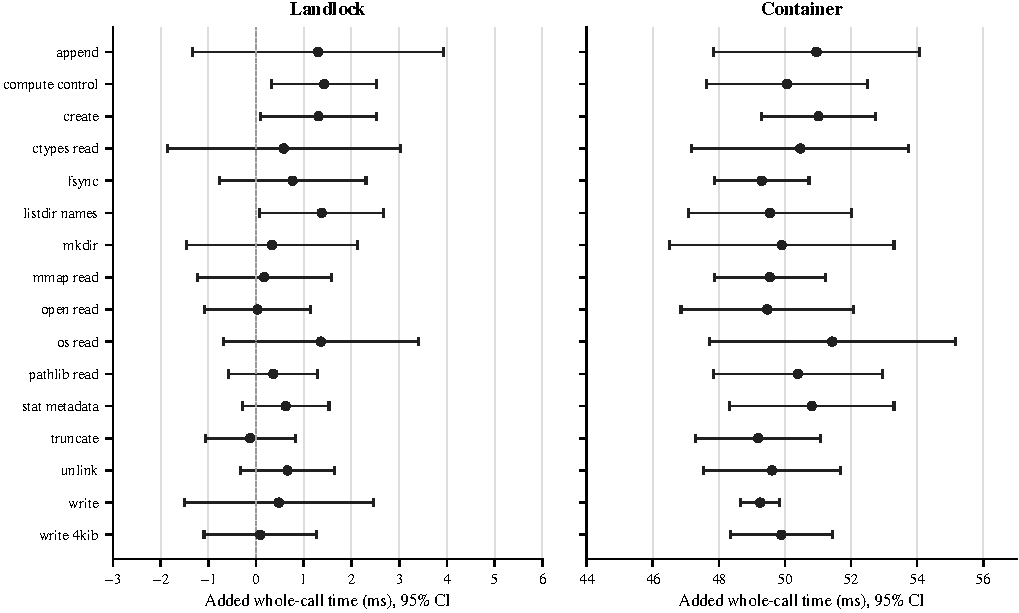
\includegraphics[width=\textwidth]{figures/operation-overhead.pdf}
  \caption{Whole-call overhead across 16 successful operation/API variants.
  Bars show $(\text{host/Python}-1)\times100\%$. Whiskers show the SD of the
  paired added duration divided by that variant's fixed Python mean, in percent;
  they are not confidence intervals. These costs include fresh-worker and policy
  work, not just the operation body or a syscall.}
  \label{fig:operation-overhead}
\end{figure*}

\subsection{Operation census and outcome classification}

The fixed census uses hidden, read-only, and writable surfaces across 49
forbidden operation/surface cases. Trusted and synthetic language-helper
baselines reproduce every effect in all three repetitions. Each of the host and
host-plus-helper conditions has 147 forbidden trials: 135 explicit denials,
six generic SQLite errors, and six empty/absent outcomes. No forbidden effect
is observed. Only 45 of the 49 cases establish explicit blocking; generic
failures and empty results are not assigned that label. Both host conditions
retain 30/30 positive-control trials. Repetitions measure stability, not
additional distinct attacks or a population attack-success rate.

The synthetic direct-language frontend rejects 27/30 controls. Its zero effects
cannot demonstrate useful complete mediation. It is not the source-verified
production mode used in the separate comparison below. The census's older,
unrestricted-affinity timings mix successful and rejected operations and are
not reused as runtime-overhead estimates. The per-case matrix and
\path{eval/ISOLATION.md} retain unsupported operations and outcome evidence.

\subsection{Matched runtime and stage attribution}

Arithmetic, an allowed canary-file read, and an allowed 4~KiB write each run in
four conditions. Each condition/workload has one retained first-use call, ten
warm-ups, and 100 measured calls. Conditions are shuffled within paired rounds
using seed 20261026. Every timing sample passes the same positive oracle.
Executor construction/preflight is timed separately; each invocation launches a
fresh worker. There is no model or durable audit sink in this cohort.
Table~\ref{tab:backend-timing} retains the reported absolute statistics, and
Table~\ref{tab:backend-paired} retains paired differences. Their SDs describe
sequential within-host variation, not independent application tasks.



Instrumentation wraps production methods without changing enforcement. The
exclusive host partition contains policy filtering, attestation, grant
compilation, negotiation, worker execution/supervision, outside-invoke time,
and an other-invoke residual. The residual is not a separately measured mechanism.
The policy stage includes file serialization, Cedar CLI validation, and an
authorization subprocess for each evaluated rule. Worker time includes launch,
confinement activation, execution, result handling, and teardown. No stage is
added to an enclosing span. Policy and worker spans have the largest stage SDs,
but their variances cannot be summed because fluctuations can be correlated.

Host setup/preflight means are 30.52, 30.72, and 30.61~ms for arithmetic, read,
and write, with SDs 2.51, 2.46, and 2.93~ms. They remain outside dispatch timing.
Instrumentation costs are included; no uninstrumented performance is inferred.
The report's full stage statistics and combined-condition measurements remain
separate from the application's 100-call replay and 20-call audit diagnostic.

\subsection{Production language and host modes}

The verified condition uses \code{cedar\_security} admission, runtime binding
validation, and grant-checked \code{read\_text}. Both conditions use real Cedar
authorization, with different policy frontends. Executors are reused and host
workers are fresh. Five warm-ups precede 50 paired successful samples per
workload. Setup and static admission are timed separately in the cohort report.
Table~\ref{tab:verified-timing} reports the dispatch comparison. The three read
sizes are workload variants of one monitored API, not three APIs.


Raw API probes from the 16-operation experiment are also submitted to the
actual verifier, with rejection diagnostics retained. Rejected operations are
assigned no successful-operation runtime. The measured production comparison
does not constitute a broad typed-resource port or a verified-mode application
integration.

\subsection{Per-operation overhead}

Sixteen operation/API variants receive five warm-ups and 50 matched samples.
Every operation must succeed in both the plain Python subprocess and host
conditions. Figure~\ref{fig:operation-overhead} normalizes each reported ratio
and the SD of its paired increment by that operation's fixed baseline mean.
Each host invocation starts a fresh worker. The baseline is neither statically
verified language execution nor the Pandas application sandbox.


A separate inner timer covers operation statements after imports, excluding
compilation, process startup, policy evaluation, and transport. It still
includes Python wrappers, open/close, and user-space work, so it is not pure
syscall time. Unsupported child-exec chains, network operations, and metadata
mutations remain explicit in the cohort report.

\paragraph{Reproduction records.}
The runtime cohort retains \path{plan.json}, \path{host-before.json},
\path{samples.jsonl}, \path{summary.json}, and \path{sources.tar.gz}.
The operation cohort adds full-precision \path{operations.csv}; the production
comparison retains admission diagnostics, setup costs, and policy/execution
breakdowns. \path{eval/scripts/paper_evaluation.py} recomputes named frozen
cohorts and writes input hashes to \path{evaluation-metrics.json}. The raw
records and exact implementation archives must accompany the artifact.
The manuscript figures use reported aggregates and preserve their source hashes;
no raw distribution or IID uncertainty estimate is synthesized from summaries.
